\documentclass[titlepage]{article}
\usepackage{babel}
\usepackage{amsmath}
\usepackage{amssymb}
\usepackage{amsthm}
\usepackage{multicol} %spalten in seite
\usepackage{graphicx} %bilder einfügen
\usepackage[normalem]{ulem} %durchstreichen
\usepackage{tabto} %tabulator mit \tab
\usepackage{hyperref}
\usepackage{tikz}
\usetikzlibrary{shapes.geometric}
\usepackage{wasysym}
\usepackage{bbm}
\usepackage{bbold}
\usepackage{xcolor}
\usepackage[T1]{fontenc}
\usepackage{mathrsfs}  
\usepackage[utf8]{inputenc}
\usepackage{listings} %quellcode
\pagestyle{plain}
\pagenumbering{arabic}
\renewcommand{\arraystretch}{1.3} %vertikaler abstand von tabellen
\newcommand{\n}{\newline}
\usepackage[left=20mm, right=15mm, top=25mm, bottom=7mm, paper=a4paper]{geometry}
\renewcommand{\contentsname}{Inhaltsverzeichnis}

\theoremstyle{plain}
\newtheorem{theorem}{Sei}
\newtheorem{theorem2}{Sei}
\newtheorem{theorem3}{Sei}
\newtheorem*{theorem4}{Sei}
\newtheorem{theorem5}{Fall}

\newcommand{\K}{\mathbb{K}}
\newcommand{\C}{\mathbb{C}}
\newcommand{\N}{\mathbb{N}}
\newcommand{\Q}{\mathbb{Q}}
\newcommand{\R}{\mathbb{R}}
\newcommand{\1}{\mathbb{1}}
\newcommand{\0}{\mathbb{0}}
\newcommand{\Z}{\mathbb{Z}}

\begin{document}
	
	\begin{center}
		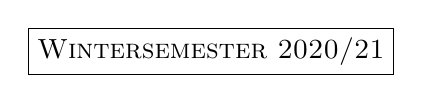
\begin{tikzpicture}
			\draw (0,0) node[draw, rectangle]{\textsc{Wintersemester 2020/21}};
		\end{tikzpicture}
		\hrulefill\\
		\begin{center}
			\LARGE\textsc{Diskrete Strukturen - Übung 10} \normalsize\\
		\end{center}
		\hrulefill
		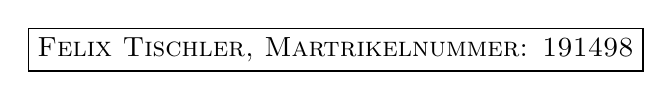
\begin{tikzpicture}
			\draw (0,0) node[draw, rectangle]{\textsc{Felix Tischler, Martrikelnummer: 191498}};
		\end{tikzpicture}
		\date{\today}
	\end{center}
	
	\part*{Relationen}
	\section*{1.)}
		\paragraph{a)}R ist asymmetrisch genau dann, wenn R irreflexiv und antisymmetrisch ist. \\ Formeller: $(xRy\land\lnot(yRx))\leftrightarrow(\lnot(xRx)\land((xRy\land yRx)\rightarrow x=y))$
		\begin{theorem}
			$xRy\land\lnot(yRx)$
		\end{theorem}
		\begin{proof}[$"\rightarrow"$]
			Für Fall $x=y$ folgt aus 1. $xRx\land\lnot(xRx)\rightarrow$\textit{ R ist irreflexiv.}
			$xRy\land yRx$ kann nicht gelten für $x\neq y$ wegen 1., somit muss $(xRy\land yRx)\rightarrow x=y$ gelten $\rightarrow$\textit{ R ist antisymmetrisch.}
		\end{proof}
		\begin{theorem}
			$\underbrace{\lnot(xRx)}_{\kappa}\land\underbrace{((xRy\land yRx)\rightarrow x=y)}_{\varkappa}$
		\end{theorem}
		\begin{proof}[$"\leftarrow"$]
			$xRy\overset{\kappa}{\rightarrow} x\neq y\overset{\varkappa}{\rightarrow}\lnot(yRx)$
		\end{proof}
		\paragraph{b)}Wenn R symmetrisch und antisymmetrisch ist, dann ist R auch transitiv. \\ Formeller: $(xRy\rightarrow yRx)\land((xRy\land yRx)\rightarrow x=y)\rightarrow(((xRy)\land(yRz))\rightarrow xRz)$
		\begin{theorem2}
			$\underbrace{(xRy\rightarrow yRx)}_{\gamma}\land\underbrace{((xRy\land yRx)\rightarrow x=y)}_{\varGamma}$
		\end{theorem2}
		\begin{proof}[Beweis:]
			$xRy\land yRx\overset{\gamma}{\rightarrow}xRy\land yRx\land yRz\land zRy\overset{\varGamma}{\rightarrow}x=y\land y=z\rightarrow x=y=z\rightarrow xRz$
		\end{proof}
		\paragraph{c)}Wenn R transitiv und irreflexiv ist, dann ist R auch asymmetrisch.
		\\ Formeller: $(((xRy\land yRz)\rightarrow xRz)\land(\lnot(xRx)))\rightarrow(xRy\rightarrow\lnot(yRx))$
		\begin{theorem3}
			$\underbrace{((xRy\land yRz)\rightarrow xRz)}_{\omega}\land\underbrace{(\lnot(xRx))}_{\varOmega}$
		\end{theorem3}
		\begin{proof}[Beweis:]
			$\underbrace{Sei}_*$ $xRy\overset{\omega}{\rightarrow}xRy\land yRx\rightarrow xRx\overset{\varOmega}{\rightarrow}\lnot(xRx). I_{\beta}(xRy)\overset{*}{=}1\land I_{\beta}(yRx)=?\rightarrow I_{\beta}(xRx)\overset{\varOmega}{=}0$. Da aus Wahr nicht Falsch folgen kann muss $I_{\beta}(yRx)=0$ sein.
		\end{proof}
	\section*{2.)}
		\paragraph{a)}
		\begin{theorem4}
			$((n,m),(k,l))\in R\Leftrightarrow n+l=m+k.$
		\end{theorem4}
		\begin{proof}[Reflexivität:]
			$(n,m)R(n,m)\Leftrightarrow n+m=m+n$
		\end{proof}
		\begin{proof}[Symmetrie:]
			$(n,m)R(k,l)\Leftrightarrow n+l=m+k\overset{kommu.}{\Longleftrightarrow} k+m=l+n\Leftrightarrow(k,l)R(n,m)$
		\end{proof}
		\begin{proof}[Transitivität:]
			$(n,m)R(l,k)\land(l,k)R(e,f)\Leftrightarrow (n+k=m+l)\land(l+f=k+e)\\\Leftrightarrow(k-l=m-n)\land(k-l=f-e)\overset{Einsetzen}{\Longrightarrow}m-n=f-e\Leftrightarrow m+e=f+n\Leftrightarrow n+f=m+e$
		\end{proof}
		\paragraph{b)}
		\paragraph{Äquivalenzklassen}
		\begin{theorem5}
			$n=m\rightarrow n+l=n+k\Leftrightarrow l=k\Rightarrow\forall n\in \N:[(n,n)]_R=\{(k,k)\mid k\in\N\}$
		\end{theorem5}
		\begin{theorem5}
			$n\neq m\Leftrightarrow n+l=m+k\Rightarrow[(n,m)]_R=\{(k,l)\mid n+l=m+k\}$
		\end{theorem5}
		\paragraph{Faktormenge}
			$M/_R=\{[(n,n)],[(n,m)]\}$
	\section*{3.)}
		\paragraph{a)} $|\mathscr{P}(M\times M)|=2^{|M|\cdot|M|}=2^{5\cdot5}=2^{25}$
		\paragraph{b)} In einer binären, reflexiven Relation sind immer diejenigen Paare $(a,b)$ enthalten die $a=b$ erfüllen. Alle anderen Elemente können 0 oder 1 annehmen, somit ist die Anzahl der unbekannten zu ermitteln welche in der Tabelle durch x visualisiert werden.
		\begin{table}[h]
			\begin{tabular}{c|ccccc}
				&$M_1$&$M_2$&$M_3$&$M_4$&$M_5$\\\hline
				$M_1$&1&x&x&x&x\\
				$M_2$&x&1&x&x&x\\
				$M_3$&x&x&1&x&x\\
				$M_4$&x&x&x&1&x\\
				$M_5$&x&x&x&x&1
			\end{tabular}
		\end{table}
	
		D.h. $5^2-5=20$ Möglichkeiten $\Rightarrow2^20$ reflexive Relationen. Dies gilt auch für irreflexive Relationen, hierbei werden die 1en durch 0en ersetzt.
		\paragraph{c)} Die Gesamtanzahl minus die reflexiven und irreflexiven Relationen.s
		$2^{25}-2\cdot2^{20}=2^{25}-2^{21}$
		\paragraph{d)} Im symmetrischen Fall kann die Relation alle geordneten Paare auf der Diagonale enthalten sowie entweder beliebig viele Elemente oberhalb oder unterhalb der Diagonalen. Je nach dem welcher Fall eintritt, nehmen die y den Wert des bezüglich an der Diagonalen gespiegelten x an. 
		\begin{table}[h]
			\begin{tabular}{c|ccccc}
				\textit{Oberhalb}&$M_1$&$M_2$&$M_3$&$M_4$&$M_5$\\\hline
				$M_1$&x&y&y&y&y\\
				$M_2$&x&x&y&y&y\\
				$M_3$&x&x&x&y&y\\
				$M_4$&x&x&x&x&y\\
				$M_5$&x&x&x&x&x
			\end{tabular}
			\begin{tabular}{c|ccccc}
				\textit{Unterhalb}&$M_1$&$M_2$&$M_3$&$M_4$&$M_5$\\\hline
				$M_1$&x&x&x&x&x\\
				$M_2$&y&x&x&x&x\\
				$M_3$&y&y&x&x&x\\
				$M_4$&y&y&y&x&x\\
				$M_5$&y&y&y&y&x
			\end{tabular}
		\end{table}
		
		Wieder ist die Anzahl der Unbekannten (x) relevant. $(25-5)/2+5=15\Rightarrow2^{15}$ Relationen.
	
		\paragraph{e)} Der Unterschied zur Symmetrie ist, dass die Diagonale mit 1 besetzt ist. 
			\begin{table}[h]
				\begin{tabular}{c|ccccc}
					\textit{Oberhalb}&$M_1$&$M_2$&$M_3$&$M_4$&$M_5$\\\hline
					$M_1$&1&y&y&y&y\\
					$M_2$&x&1&y&y&y\\
					$M_3$&x&x&1&y&y\\
					$M_4$&x&x&x&1&y\\
					$M_5$&x&x&x&x&1
				\end{tabular}
				\begin{tabular}{c|ccccc}
					\textit{Unterhalb}&$M_1$&$M_2$&$M_3$&$M_4$&$M_5$\\\hline
					$M_1$&1&x&x&x&x\\
					$M_2$&y&1&x&x&x\\
					$M_3$&y&y&1&x&x\\
					$M_4$&y&y&y&1&x\\
					$M_5$&y&y&y&y&1
				\end{tabular}
			\end{table}
		
		Die Anzahl der Unbekannten verringert sich dementsprechend. $(25-5)/2=10\Rightarrow 2^{10}$ Relationen.
	
\end{document}
